%%%%%%%%%%%%%%%%%%%%%%%%%%%%%%%%%
%
%       EXERCÍCIO
%
%%%%%%%%%%%%%%%%%%%%%%%%%%%%%%%%%

\ifdefstring{\atividade}{prova}{%
    \ifdefstring{\modo}{objetivo}{%
        \renewcommand{\valorquestao}{\ValorQObj\ ponto}
    }{%
        \renewcommand{\valorquestao}{\ValorQDisc\ pontos}
    }%
}%

\begin{exercicioBanco}[\valorquestao]
Determine o gráfico da função \(f(x) = |x| + |x+1| - |x-1|\).

% Define as alternativas
\newcommand{\alternativas}{%
    \begin{center}
    \begin{tabular}{C{20pt}C{140pt}C{20pt}C{140pt}C{20pt}C{140pt}}
        (a) 
        &
        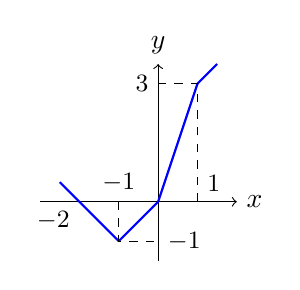
\begin{tikzpicture}[scale=0.5]
            % Eixos
            \draw[->] (-3,0) -- (2,0) node[right] {\(x\)};
            \draw[->] (0,-1.5) -- (0,3.5) node[above] {\(y\)};

            % Gráfico da função f(x) = |x| + |x+1| - |x-1|
            \draw[domain=-2.5:-1, thick, blue] plot (\x, {-\x - 2}); % x < -1
            \draw[domain=-1:0, thick, blue] plot (\x, {\x});    % -1 \le x < 0
            \draw[domain=0:1, thick, blue] plot (\x, {3*\x});    % 0 \le x < 1
            \draw[domain=1:1.5, thick, blue] plot (\x, {\x+2});    % x \ge 1

            % Marcações das raízes
            \node[below left] at (-2,0) {\small\(-2\)};

            % Marcação do vértice (x = -1)
            \draw[dashed] (-1,0) -- (-1,-1) -- (0,-1);
            \node[above] at (-1,0) {\small\(-1\)};
            \node[right] at (0,-1) {\small\(-1\)};
            
            \draw[dashed] (1,0) -- (1,3) -- (0,3);
            \node[above right] at (1,0) {\small\(1\)};
            \node[left] at (0,3) {\small\(3\)};
        \end{tikzpicture}
        &
        (b) 
        &
        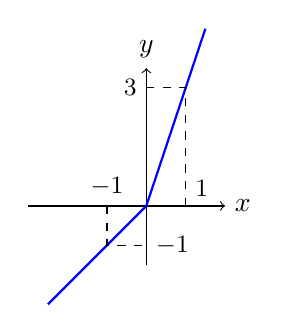
\begin{tikzpicture}[scale=0.5]
            % Eixos
            \draw[->] (-3,0) -- (2,0) node[right] {\(x\)};
            \draw[->] (0,-1.5) -- (0,3.5) node[above] {\(y\)};

            % Gráfico incorreto
            \draw[domain=-2.5:0, thick, blue] plot (\x, {\x});
            \draw[domain=0:1.5, thick, blue] plot (\x, {3*\x});

            % Guias
            \draw[dashed] (-1,0) -- (-1,-1) -- (0,-1);
            \draw[dashed] (1,0) -- (1,3) -- (0,3);

            % Marcações
            \node[above] at (-1,0) {\small\(-1\)};
            \node[right] at (0,-1) {\small\(-1\)};
            \node[above right] at (1,0) {\small\(1\)};
            \node[left] at (0,3) {\small\(3\)};
        \end{tikzpicture}
        &
        (c)
        &
        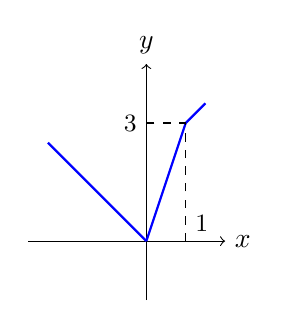
\begin{tikzpicture}[scale=0.5]
            % Eixos
            \draw[->] (-3,0) -- (2,0) node[right] {\(x\)};
            \draw[->] (0,-1.5) -- (0,4.5) node[above] {\(y\)};

            % Gráfico incorreto
            \draw[domain=-2.5:0, thick, blue] plot (\x, {-\x});
            \draw[domain=0:1, thick, blue] plot (\x, {3*\x});
            \draw[domain=1:1.5, thick, blue] plot (\x, {\x + 2});

            % Guias
            \draw[dashed] (1,0) -- (1,3) -- (0,3);

            % Marcações
            \node[above right] at (1,0) {\small\(1\)};
            \node[left] at (0,3) {\small\(3\)};
        \end{tikzpicture}
        \\
        (d)
        &
        \begin{tikzpicture}[scale=0.5]
            % Eixos
            \draw[->] (-3,0) -- (2,0) node[right] {\(x\)};
            \draw[->] (0,-2.5) -- (0,3.5) node[above] {\(y\)};

            % Gráfico incorreto
            \draw[domain=-2.5:-1, thick, blue] plot (\x, {-\x - 2});
            \draw[domain=-1:1, thick, blue] plot (\x, {-1});
            \draw[domain=1:1.5, thick, blue] plot (\x, {4*\x - 5});

            % Guias
            \draw[dashed] (-1,0) -- (-1,-1) -- (0,-1);
            \draw[dashed] (1,0) -- (1,-1) -- (0,-1);

            % Marcações
            \node[below left] at (-2,0) {\small\(-2\)};
            \node[above] at (-1,0) {\small\(-1\)};
            \node[above left] at (1,0) {\small\(1\)};
            \node[below right] at (0,-1) {\small\(-1\)};
        \end{tikzpicture}
        &
        (e) 
        &
        \begin{tikzpicture}[scale=0.5]
            % Eixos
            \draw[->] (-3,0) -- (2,0) node[right] {\(x\)};
            \draw[->] (0,-1.5) -- (0,4.5) node[above] {\(y\)};

            % Gráfico incorreto
            \draw[domain=-1.5:1, thick, blue] plot (\x, {1.5*\x + 1.5});
            \draw[domain=1:1.5, thick, blue] plot (\x, {3});

            % Guias
            \draw[dashed] (1,0) -- (1,3) -- (0,3);

            % Marcações
            \node[above left] at (-1,0) {\small\(-1\)};
            \node[above right] at (1,0) {\small\(1\)};
            \node[left] at (0,3) {\small\(3\)};
        \end{tikzpicture}
        &&
    \end{tabular}
\end{center}
%
}

% Define a resposta correta
\newcommand{\resposta}{A}

% Lógica condicional para exibição
\ifdefstring{\atividade}{lista}{%
    \alternativas
    \vspace{0.5em}
    
    \noindent\textbf{Resposta:} letra \textbf{\resposta}.
}{%
    \ifdefstring{\modo}{objetivo}{%
        \alternativas
    }{%
        % modo = discursiva → não mostra alternativas
    }
}
\end{exercicioBanco}

